\documentclass[10pt]{notes}
 \usepackage{wasysym}
\begin{document}


%%%%%% Writing big font size title %%%%%
% \title{\textbf{ST101: Introduction to Statistics\\Homework 1}}
% \author{By Zhu Xuelin\tmemail{xuelin@u.nus.edu}}
% \date{}
% \maketitle

%%%%%% Writing small font size title %%%%%
% \title{\large Customed Notes Template}
% \author{\normalsize \href{mailto:xuelin@u.nus.edu}{Zhu Xuelin}}
% \date{}
% \maketitle

%%%%%% Writing title with header %%%%%
\thispagestyle{firstpage}


\begin{center}
    \large 线性回归$\to$局部回归
\end{center}

\begin{setup}
    已收集到$(x_i,y_i)_{i=1}^n$数据样本，并观察到$x$与$y$之间以某个函数$y\approx f(x)$关系相连。我们想要估计该函数。
\end{setup}

\noindent
回顾参数回归方法：
\begin{itemize}
    \item 线性回归: 如果该函数看起来像线性，我们可以假设 $f(x)=\beta_0+\beta_1 x$，再通过最小化$L_2$损失得到线性模型：
    \begin{align}
        \min_{f(x)} \left\{\sum_{i=1}^{n} \Big[y_i-f(x_i)\Big]^2\right\} = \min_{\beta_0,\beta_1} \left\{\sum_{i=1}^{n} \Big[y_i-(\beta_0+\beta_1 x_i)\Big]^2\right\}.
        \label{eq-l2-loss-lm}
    \end{align}
    \item 多项式回归：如果该函数并不像线性，可以假设$f(x)=\beta_0+\beta_1 x+\cdots+\beta_p x^p$，同样最小化$L_2$损失。
    % \item Splines-based回归（如果没见过，就请把它理解为几个固定的变换）: 设置$p$个已知变换 $N_1(x),\dots,N_p(x)$，采用 $f(x)=\beta_0+\beta_1 N_1(x)+\cdots+\beta_p N_p(x)$，同样最小化$L_2$损失。我们甚至可以引入$L_1$ or $L_2$惩罚项，来控制估计量$\hat{f}$的平滑/过拟合程度。
\end{itemize}
\noindent 
无论采用以上哪种方法，最小化$\min_{f(x)}$都可以被化简为求解有限个参数的$\min_{\beta_0,\dots,\beta_p}$问题。我们并没有在无限大的函数空间中寻找最优解，这让计算量始终在可控范围之内（nice \smiley）。而且以上方法一旦得到参数估计$\hat{\beta}$，我们就不再需要原始数据$(x_i,y_i)_{i=1}^n$来做未来预测，仅使用$\hat{\beta}$就可以。这也是他们作为参数方法的好处之一。
% 这两个特征是很重要的，一会我们会看到：局部回归方法并不能被化简为有限参数，所以计算量巨大。以及对于任何未来预测，我们都需要全部样本重新计算。

\subsection{局部回归方法}
我们格外注意损失函数(\ref{eq-l2-loss-lm})：以上方法给所有的样本$i\in [n]$都分配了相同的权重。而局部回归方法是另一套逻辑：固定一个点$x\in\bbR$（我们不妨称待估点），我们想估计待估点的函数值$f(x)$，那么我们就去看$x$附近有哪些样本。离$x$越近的样本，我就在损失函数中给他更高的权重。

\subsubsection{$k$-NN回归}
以上思路最直接的落地方法就是$k$-NN，即$\hat{f}(x)\leftarrow$ 距离待估点最近的$k$个样本的response平均值，可以写成：
\begin{align*}
    \hat{f}(x)=\sum_{i=1}^n w_i(x)y_i,\quad
    \text{其中}
    w_i(x)=
    \begin{cases}
        1/k & \text{若$x_i$是距离$x$最近的$k$个样本，} \\ 
        0 & \text{若$x_i$不是。}
 \end{cases}
\end{align*}
这里的$w_i(x)$正表示第$i$号样本的权重：距离待估点$x$越近，第$i$号样本权重$w_i(x)$更高。

\begin{center}
    \begin{minipage}[t]{0.42\textwidth}
        \vspace{0pt}
        \centering
        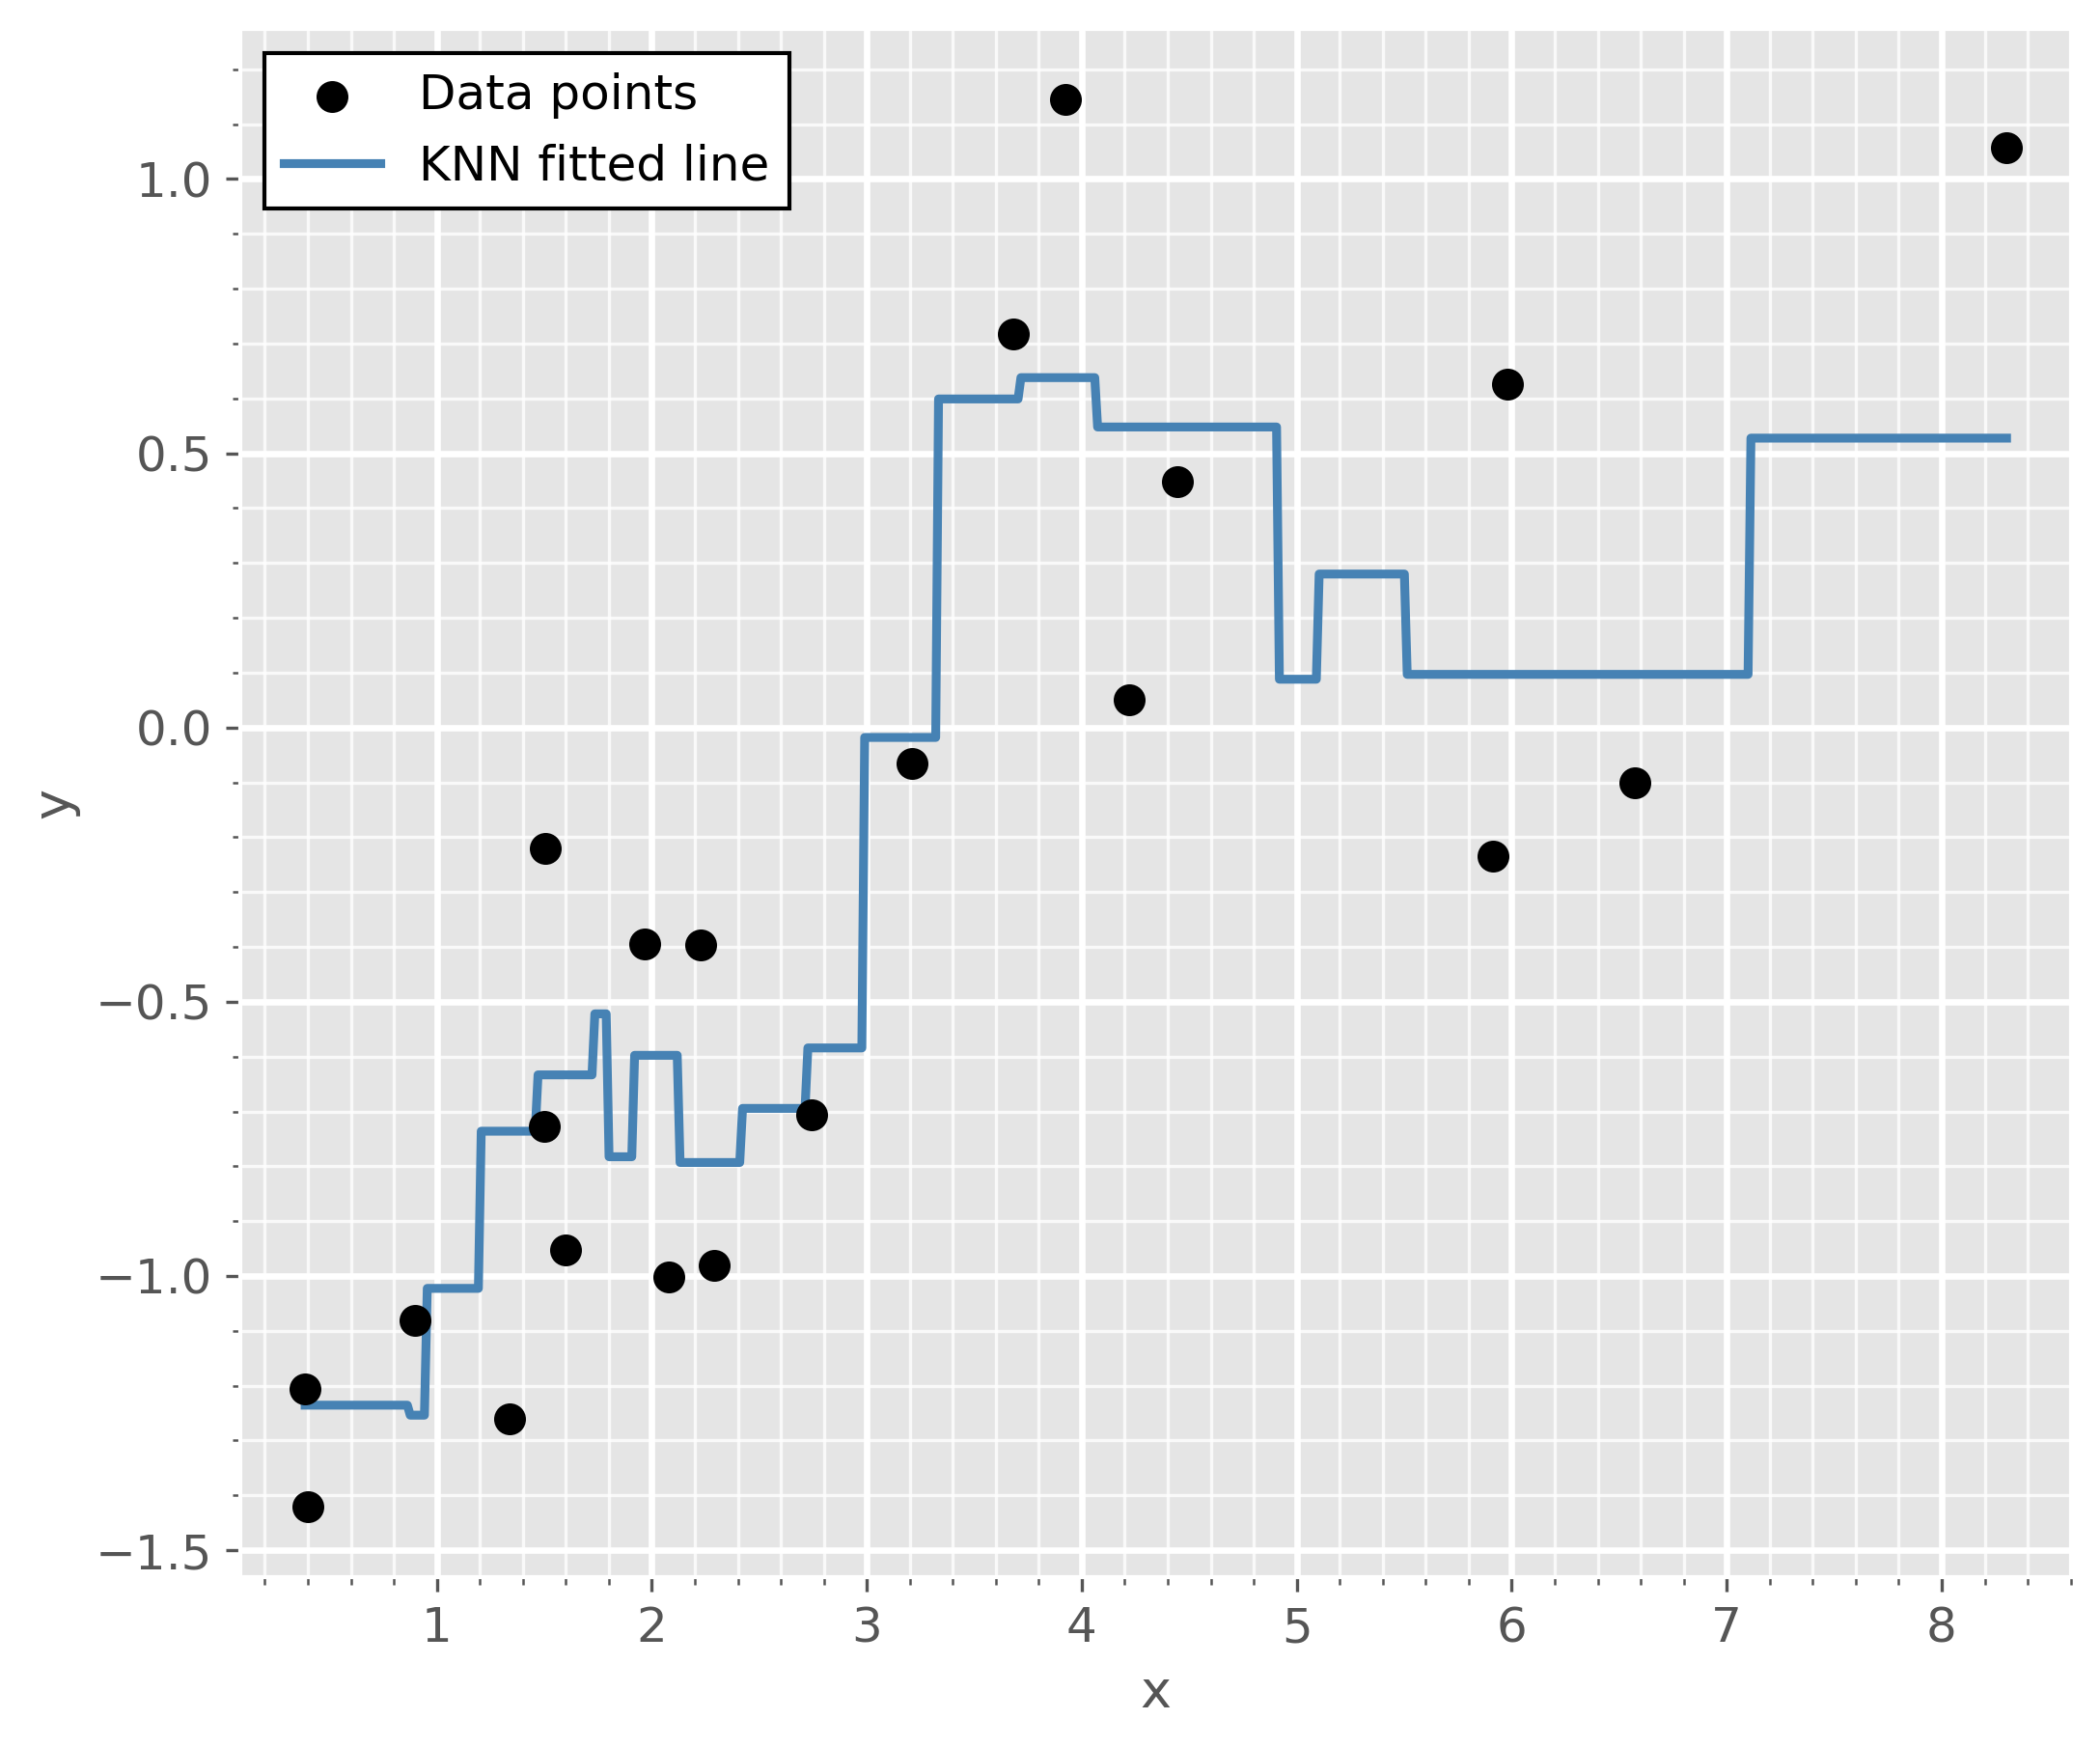
\includegraphics[width=\textwidth]{knn-reg.png}
    \end{minipage}\hfill
    \begin{minipage}[t]{0.52\textwidth}
        \vspace{4pt}
        左侧是一个$k$-NN回归的例子。在计算蓝色拟合线$\hat{f}(x)$时，我们别无他法，只能逐点计算：
        \begin{itemize}
            \item 固定待估点$x=0.1$，找到距离$x=0.1$最近的$k$个样本，计算他们response的平均值，并赋为$\hat{f}(0.1)$；
            \item 待估点向右移动一点点，比如$x=0.2$，计算$\hat{f}(0.2)$ $\cdots\cdots$ 直到完成整个蓝色曲线。
        \end{itemize}
        如果我们固定一个样本$i$，把观察权重$w_i(x)$作为一个$x$的函数来观察，可以发现$w_1(x),\dots,w_n(x)$每一个都不是连续函数。所以他们的线性组合$\hat{f}(x)$，作为$x$的函数，也是不连续的。这也符合我们看到左侧蓝色拟合线有跳点的现象。
    \end{minipage}
\end{center}

所以，我们总结$k$-NN回归：他可以写成$\hat{f}(x)=\sum_{i=1}^n w_i(x)y_i$的形式；拟合$\hat{f}(x)$的计算量很大，因为只能不停移动待估点、一个点一个点地去算；由于$w_i(x)$选择了不连续函数，所以$\hat{f}(x)$也是不连续的。

第一点特征，正是它被归类为局部回归方法的原因 —— 在待估点附近的局部样本拥有更大的权重。后面我们会介绍的几种局部回归都有$\hat{f}(x)=\sum_{i=1}^n w_i(x)y_i$的形式。第二点特征，也会被我们后续介绍的所有local regression方法给继承：他们都得逐点计算，比起参数方法，计算量巨大（bad \frownie）。而第三点，是我们为什么要从$k$-NN升级原因 —— 我们想要连续函数！

\subsubsection{核回归（Kernel Regression）}
为了得到一个连续函数$\hat{f}(x)$，在$k$-NN基础上不难发现，我们其实只需要把所有权重函数$w_i(x)$都换成关于$x$连续的就可以。
那什么样的函数$w_i(x)$既能够作为权重使用（在$x$附近更大、远离$x$时变小），又能给我们很好的连续性呢？正态分布的钟形曲线！
\vspace{-1em}
\begin{center}
    \begin{minipage}[t]{0.45\textwidth}
        \vspace{0pt}
        \centering
        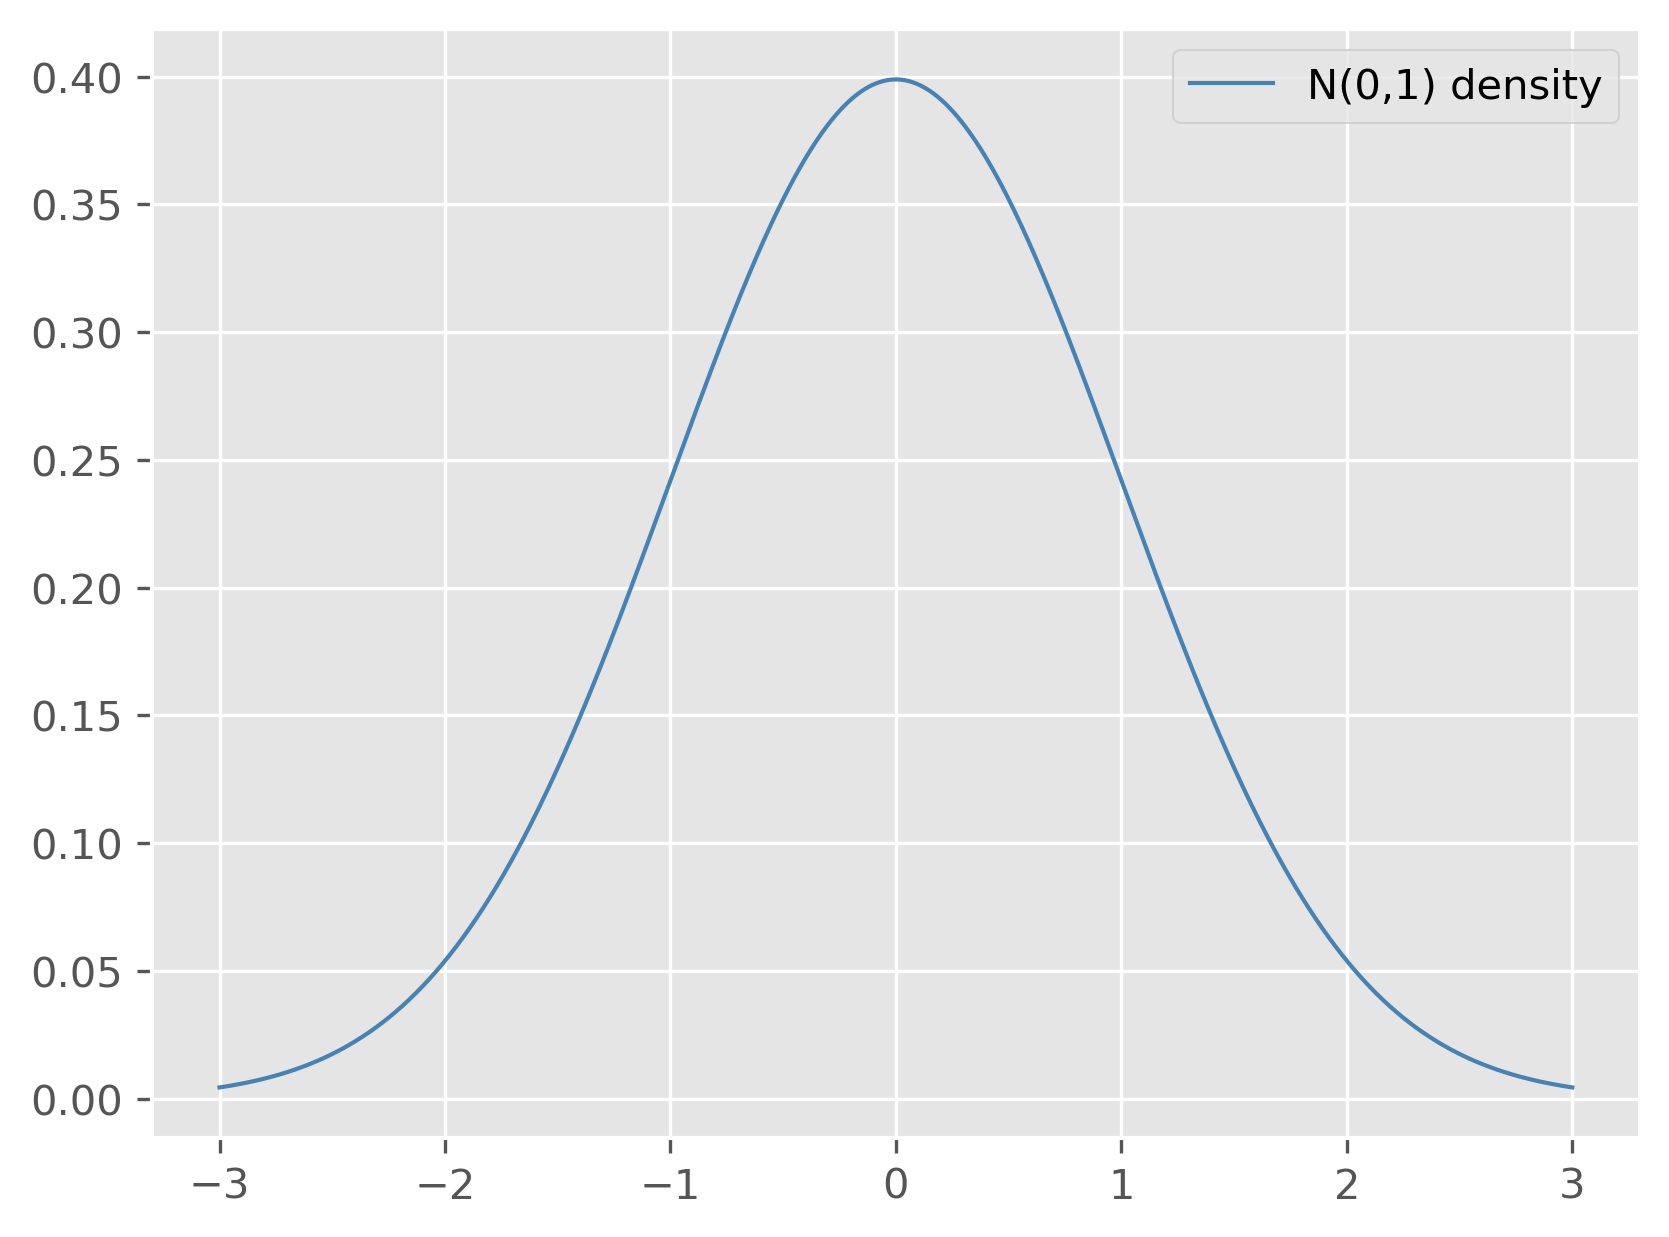
\includegraphics[width=\textwidth]{normal-density.png}
    \end{minipage}\hfill
    \begin{minipage}[t]{0.52\textwidth}
        \vspace{4pt}
        如果对每个样本$i$都采用权重$$w_i(x)=\frac{1}{\sqrt{2\pi}}\exp{\{(x-x_i)^2\}},$$
        那么只有待估点$x$局部附近的样本会有相当高的权重，而很远的样本权重会快速衰减到0，所以正态密度是非常合适的候选函数。不过我们还不能直接采用它，因为它还有两个缺憾：
        \begin{itemize}
            \item 它并不带来任何参数帮助我们控制权重衰减的速度；
            \item 这个权重加起来还不是1，即$\sum_{i=1}^{n}w_i(x)\ne 1$，所以$\hat{f}(x)=\sum_{i=1}^{n}w_i(x)y_i$还不能被看作“加权平均”。
        \end{itemize}
    \end{minipage}
\end{center}

但这两个问题并不麻烦，我们把估计器$\hat{f}(x)$设置成下面的形式就可以解决：
\begin{align}
    \hat{f}(x)=\sum_{i=1}^{n}\frac{K\!\left(\frac{x-x_i}{h}\right)}{\sum_{j=1}^{n}K\!\left(\frac{x-x_j}{h}\right)}y_i,\quad
    \text{其中$K(\cdot)$是$\normal(0,1)$的密度函数，而窗宽$h$是我们预设的一个值。}
    \label{eq-kernel-reg}
\end{align}
这样一来，我们实则是把中间比较复杂的那一项看作权重：
\begin{align*}
    w_i(x)=\frac{K\!\left(\frac{x-x_i}{h}\right)}{\sum_{j=1}^{n}K\!\left(\frac{x-x_j}{h}\right)},\quad\text{它的分母其实正是一个归一化，即：现在对于任意待估点$x$都有 }
    \sum_{i=1}^{n}w_i(x)=1
    \text{。}
\end{align*}
窗宽$h$则控制权重的衰减速度：窗宽$h$越大，各个样本的权重$w_i(x)$会变得更加“均匀”（有兴趣的话，写个simulation计算看看我说的“均匀”是什么意思），导致拟合曲线整体看起来走势更平缓；而窗宽$h$越小，待估点$x$附近的样本权重会更加突出，导致拟合曲线整体随着数据的弯折更锋利。下面是一张实例图。

\begin{center}
    \begin{minipage}[t]{\textwidth}
        \vspace{0pt}
        \centering
        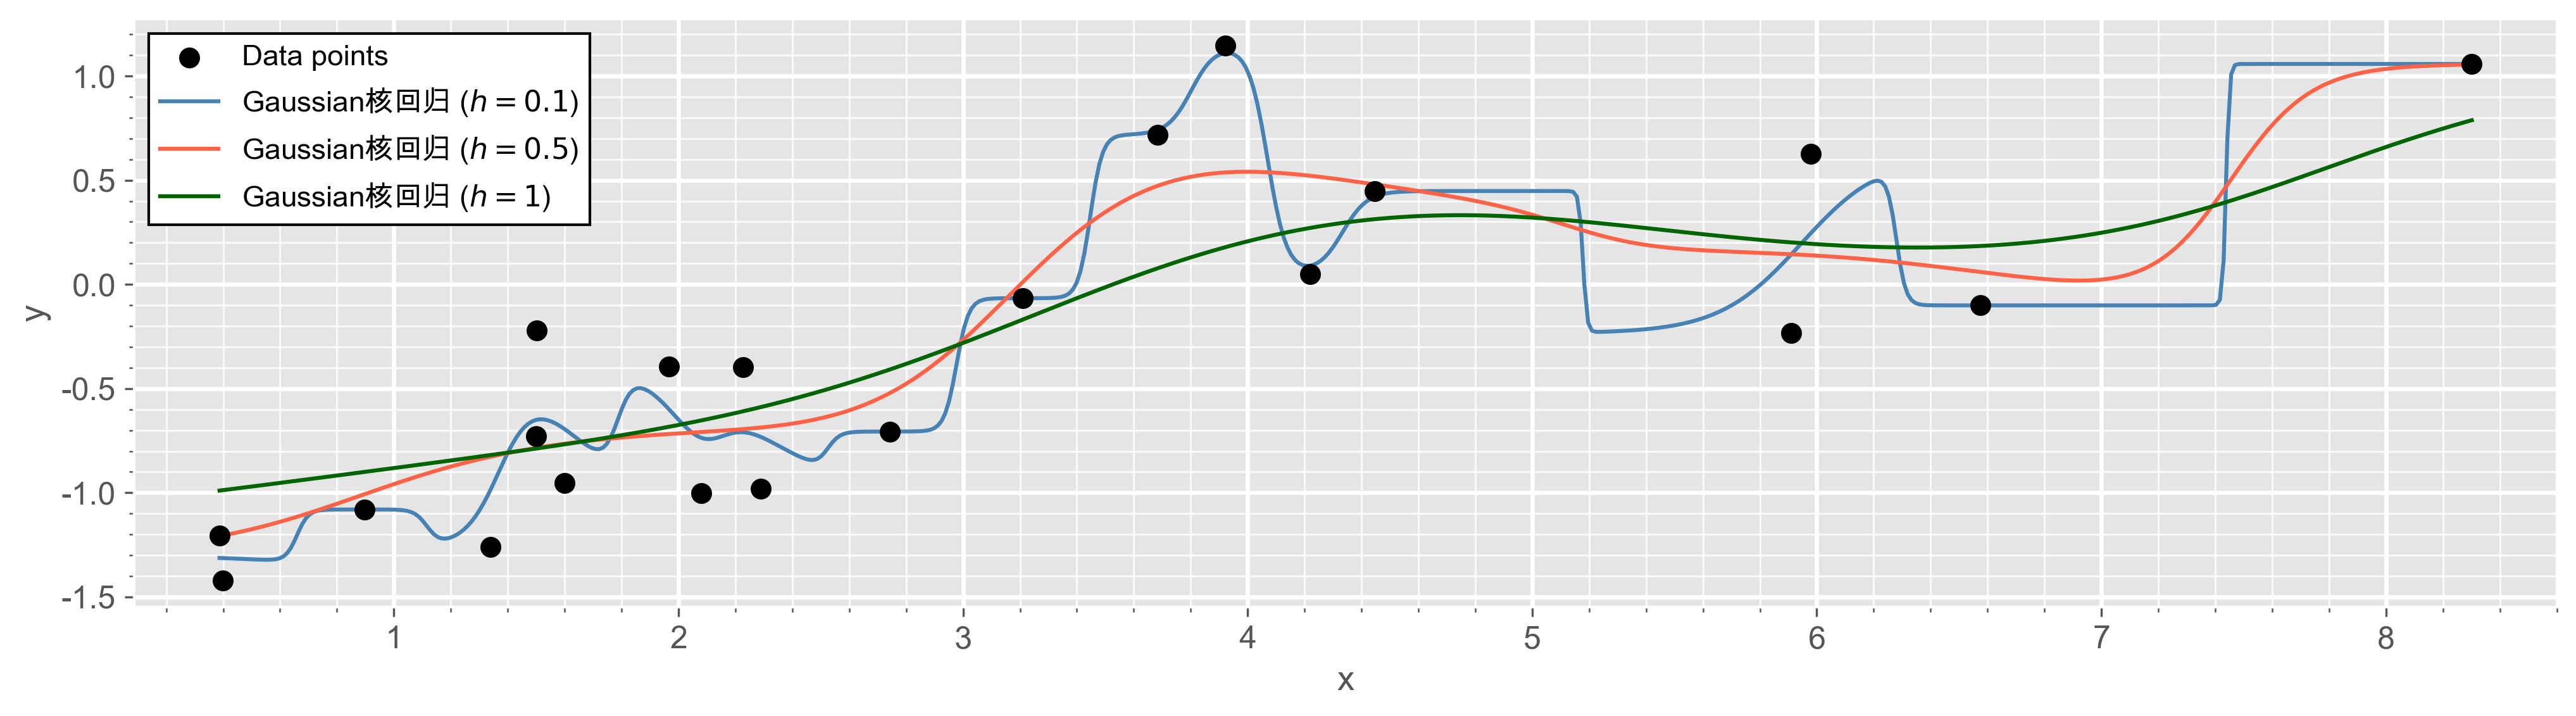
\includegraphics[width=\textwidth]{kernel-reg.png}
    \end{minipage}
\end{center}

其实采用方程(\ref{eq-kernel-reg})得到的估计器$\hat{f}$并不一定要局限于$K$为正态密度。只要$K(\cdot)$是连续的、在待估点附近的局部样本有更大的权重，都可以作为一个合适的候选，并通过$K(\cdot/h)$加入窗宽的方式控制衰减速度。所以我们把这一类函数下一个定义。
\begin{definition}[Kernel function]
    一个函数$K:\bbR\mapsto \bbR^+$，如果满足:
    \begin{align*}
        (1) \int_{-\infty}^\infty K(x)dx=1,\qquad 
        (2) \int_{-\infty}^\infty xK(x)dx=0,\qquad
        (3) \int_{-\infty}^\infty x^2 K(x)dx<\infty，
    \end{align*}
    就被称作核函数。采用方程(\ref{eq-kernel-reg})得到的估计器$\hat{f}$，也被称为核回归。
\end{definition}

\subsubsection{局部常数回归（Local Constant）}
回顾我们的任务：在样本$(x_i,y_i)_{i=1}^n$中，我们观察到$y\approx f(x)$，所以想要估计该函数。如果采用损失函数的思路，我们很自然想到最小化
$\min_{f}
\left\{\sum_{i=1}^{n}\big[y_i-f(x_i)\big]^2\right\}$，再代入$f$具体形式求解，比如$f(x_i)=\beta_0+\beta_1 x_i$，线性回归/多项式回归，我们都是这样做的。

但如前文所说，局部回归是另一套逻辑：先固定待估点$x\in\bbR$，我们的目标是估计这个单点的$f(x)$，即：逐点估计、而不是直接估出整个函数。为了适应这个目标，距离待估点更近的样本应有更大的权重。所以我们用核函数$K(\cdot)$作为权重，把原有的损失函数$\min_{f}
    \left\{\sum_{i=1}^{n}\big[y_i-f(x_i)\big]^2\right\}$升级为
\begin{align}
    \text{加权损失：}\quad 
    \min_{f}
    \left\{\sum_{i=1}^{n}K\!\left(\frac{x-x_i}{h}\right)\big[y_i-f(x_i)\big]^2\right\}\text{。}
    \label{eq-local-reg-loss}
\end{align}
但接下来如何解公式(\ref{eq-local-reg-loss})呢？我们还做不到。因为一来，我们没有给$f$设一个具体形式，所以$f(x_i)$无法代入；二来，我们想要估计的是待估点的$f(x)$，不是样本点的$f(x_i)$，而这个目标甚至还没有出现在损失函数中。为了让它出现，我们需要知道待估点的$f(x)$和样本点的$f(x_i)$之间有什么关系。这本质上，决定了我们把估计器$\hat{f}$限制成什么样子。

我们从最简单的关系开始，假设$f(x_i)\approx f(x)$，即所有的样本点$f(x_i)$都和待估点$f(x)$差不多。当然这个假设非常强，但随之它带来了很简单的推导，所以我们先从这里开始，后续再放松这个假设。我们代入这个假设的$f(x_i)\approx f(x)$进入上面的损失函数(\ref{eq-local-reg-loss})，进一步化简为
\begin{align*}
    \min_{f}
    \left\{\sum_{i=1}^{n}K\!\left(\frac{x-x_i}{h}\right)\big[y_i-f(x)\big]^2\right\}
\end{align*}
现在整个损失函数中，与$f$有关的项只有$f(x)$，而且待估点$x$在最开始就已经被固定了，这让$f(x)$只是一个未知的常数，所以不妨记$\beta_0=f(x)$。这样我们就可以用OLS的推导方式，对$\beta_0$求导、解出方程、得到
$$\hat{f}(x)=\hat{\beta}_0=\sum_{i=1}^{n}\frac{K\!\left(\frac{x-x_i}{h}\right)}{\sum_{j=1}^{n}K\!\left(\frac{x-x_j}{h}\right)}y_i.$$
这正是前文的方程(\ref{eq-kernel-reg})、核回归的显式公式。所以本质上，核回归是加权损失(\ref{eq-local-reg-loss})限制在「待估点$f(x)$和所有样本点$f(x_i)$都差不多」假设下的最优解。而这个假设，也并不用那么严格，由于权重函数$K\!\left(\frac{x-x_i}{h}\right)$的存在，远离待估点的样本在损失函数中权重几乎为0，不参与估计了，所以我们假设的其实是「待估点$f(x)$和它局部附近的样本点$f(x_i)$差不多」，
这也是他被称作局部常数回归的原因——我们求解时限制了$\hat{f}(x)$在局部为一个常数$\beta_0$（局部常数假设）。而到底多“局部”，取决于窗宽$h$的大小了。这个数值，我们一般当作超参数，和$k$-NN回归的$k$一样，通过cross-validation从实际数据中选取。
\begin{remark}
    虽然它叫局部“常数”，但拟合线$\hat{f}(x)$并不是常数、甚至不是线性。如果核函数是连续的，在核回归的讨论中我们已经得出结论、看到实例：$\hat{f}(x)$是一条曲线！
\end{remark}

\subsubsection{局部线性模型（Local Linear）}
回到我们的损失函数(\ref{eq-local-reg-loss})，
现在我们考虑局部线性假设$f(x_i)\approx f(x)+f'(x)(x_i-x)$，即：待估点$x$局部的样本可以被$f$在$x$处的切线逼近，或者简单地说，函数$f$在待估点$x$附近是一条直线。这个假设下，损失函数(\ref{eq-local-reg-loss})会写成
\begin{align*}
    \min_{f}
    \left\{\sum_{i=1}^{n}K\!\left(\frac{x-x_i}{h}\right)\Big[y_i-\big[f(x)+f'(x)(x_i-x)\big]\Big]^2\right\}.
\end{align*}
同样地，其中与$f$有关的项只有$f(x)$和$f'(x)$，我们记$\beta_0:=f(x)$和$\beta_1=f'(x)$，则我们想求解
\begin{align*}
    \min_{\beta_0,\beta_1}
    \left\{\sum_{i=1}^{n}K\!\left(\frac{x-x_i}{h}\right)\Big[y_i-\big[\beta_0+\beta_1 (x_i-x)\big]\Big]^2\right\}
    \Rightto 
    \text{挑战：\underline{你能快速想到$\hat{\bb}:=(\hat{\beta}_0,\hat{\beta}_1)^\top$的显式解吗（它有吗）？}}
\end{align*}
有的：我们把权重写成$w_i$、把$(x_i-x)$当作新的自变量$z_i$，损失函数就可以被看作$\left\{\sum_{i=1}^{n}w_i\big[y_i-(\beta_0+\beta_1 z_i)\big]^2\right\}$，它是$y\sim z$的weighted least square，所以我们只需代入WLS的公式，就可以快速解出$\hat{\bb}$。具体来说，固定待估点$x$：
\begin{enumerate}
    \item 记新的数据矩阵为$X\in\bbR^{n\times 2}$，其第一列为1，第二列为$(z_1,\dots,z_n)^\top$；记response vector为$Y=(y_1,\dots,y_n)^\top$；
    \item 算出各样本权重$K\!\left(\frac{x-x_i}{h}\right)$，记权重矩阵$W(x)=\operatorname{diag}\big[K\!\left(\frac{x-x_1}{h}\right),\dots,K\!\left(\frac{x-x_n}{h}\right)\big]$；
    \item 代入WLS公式，算出显式解$\hat{\bb}(x)=\big[X'W(x)X\big]^{-1}X'W(x)Y$；
    \item 分量$\hat{\beta}_0(x)$和$\hat{\beta}_1(x)$在$\hat{\bb}(x)$中算出。回顾他们的定义，估计器是$\hat{f}(x)=\hat{\beta}_0(x)$和副产物$\hat{f}'(x)=\hat{\beta}_1(x)$。
\end{enumerate}
这个模型就是局部线性回归（local linear regression）。我们可以很自然地扩展到局部多项式，只需要把假设修改为局部多项式逼近就好，计算方法都和局部线性回归师承一脉。

\begin{remark}
    如果我们对比线性模型（全局/常规）和局部线性模型，他们的区别在于
    \begin{itemize}
        \item 损失函数不同：针对待估点$x$，线性模型给所有样本的权重相同，而局部线性模型给更近的样本更大的权重；
        \item 这局部加权让系数$\hat{\bb}(x)$与待估点$x$本身相关，进一步导致局部线性模型拥有以下两个特征。
        \item 第一，局部线性模型本身并不是线性函数。其实不仅如此，局部常数回归就已不是线性函数，从它的显式解(\ref{eq-kernel-reg})也能看出。
        \item 第二，计算量大，因为我们只能逐点计算$\hat{f}(x)$（我们在$k$-NN已经提到过）。
    \end{itemize}
\end{remark}




\end{document}
